% $Id: introduction.tex 34630 2013-04-29 22:53:51Z roldeman $

\section{Supersymmetry Searches with the \boldmath $\alpha_T$ Variable}
\label{sec:alphaT}

As motivated in Section~2, it is important to carry out a search for SUSY at the LHC in the hadronic jets plus missing transverse energy, $\cancel{E}_T$, final state. By considering only events with an all hadronic final state, vetoing isolated leptons, electroweak backgrounds can be suppressed. This is particularly important as the only genuine source of $\cancel{E}_T$ in the SM is neutrinos.
\subsection{Definition of \boldmath $\alpha_T$}
The major problem with purely hadronic events is the huge background from multijet events. QCD events can give fake $\cancel{E}_T$ signatures if one or more of the jets are mismeasured in the detector. To overcome this, the dimensionless variable $\alpha_T$ is introduced \cite{AlphaTproposalCMS:2008vya} \cite{AlphaTproposalPhysRevLett.101.221803}. For a dijet system it is defined as:
\begin{equation}
\alpha_T=\frac{E_T^{j_2}}{M_T},
\end{equation}
where $E_T^{j_2}$ is the energy of the lowest energy jet, $M_T=\sqrt{H_T^2-\cancel{H}_T^2}$ is the invariant mass of the dijet system. It is constructed from the jet characterising variables:
\begin{equation}
H_T=\sum_{i=1}^{n_{jet}}E_T^{j_i}, 
\end{equation}
and
\begin{equation}
\cancel{H}_T=|\sum_{i=1}^{n_{jet}}\vec{p}_T^{j_i}|,
\end{equation}
with $n_{jet}$ jets, $j_i$, with transverse momentum $\vec{p}_T^{j_i}$ and transverse energy $E_T^{j_i}$. For events with more than two jets a pseudo dijet system is formed by combining jets. The system chosen is one that minimises $|\Delta H_T|$. This is the difference between the $E_T$ of each pseudo jet, where $E_T$ is the scalar sum of the transverse energies of all the jets in each pseudo jet. This leads to a generalised form of $\alpha_T$ \cite{AlphaT8TeVChatrchyan:2013lya}:
\begin{equation}
\alpha_T=\frac{1}{2}\times\frac{H_T-\Delta H_T}{\sqrt{H_T^2-\cancel{H}_T^2}}
\end{equation}
In the case that two well measured back to back jets are produced by a QCD process, assuming the mass of the jet constituents is much less than the total energy of the jet, $\alpha_T=0.5$. If one of these jets is mismeasured, resulting in fake $\cancel{E}_T$, then $\alpha_T<0.5$. However, if the two jets are recoiling from genuine $\cancel{E}_T$ then $\alpha_T>0.5$. A cut on $\alpha_T$ of around $0.55$ can remove almost all QCD background. The power of this variable to eliminate QCD background can be seen in Fig.~\ref{fig:alphaT}.
\begin{figure}
	\begin{center}
		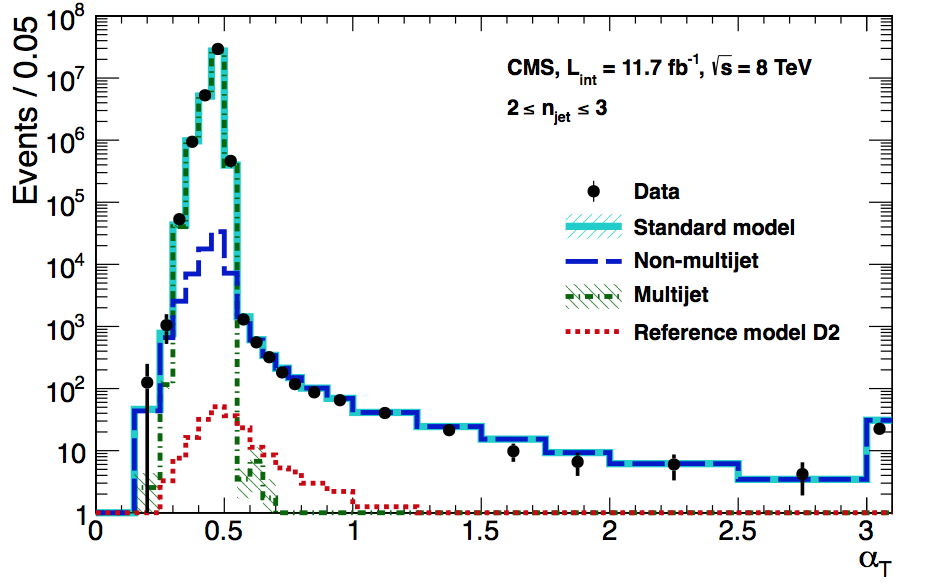
\includegraphics[width=0.8\linewidth]{alphaT1_bkgd}
	\end{center}
	\caption{The $\alpha_T$ values for events with $H_T>375$ GeV and 2 to 3 jets that pass all other cuts imposed in the $\alpha_T$ analysis. The green dotted line shows the expected multijet QCD background that can be removed with an appropriate cut on $\alpha_T$ \cite{AlphaT8TeVChatrchyan:2013lya}}
	\label{fig:alphaT}
\end{figure}
\subsection{The \boldmath $\alpha_T$ analysis}
Events are selected with at least one vertex with $p_T>50$~GeV jets, where the jets are well reconstructed in the central region, $|\eta|<3$. Events with isolated\footnote{A particle is isolated if there are no other particles within a cone of $\sqrt{(\Delta\phi)^2+(\Delta\eta)^2}=0.3$} leptons of $p_T>10$~GeV or photons of $p_T>25$~GeV are vetoed. Events are categorised based on the number of jets, the number of jets with a reconstructed b-quark and the value of $H_T$. This allows for a variable $\alpha_T$ cut based on the category, maximising signal acceptance. Full details of the analysis can be found at \cite{AlphaT8TeVChatrchyan:2013lya} and \cite{AlphaT_7TeV_PRLChatrchyan:2011zy}.
